\subsection{弧微分}
\paragraph{}
设函数$f(x)$在区间$(a,b)$内具有连续导数。在曲线$y=f(x)$上取固定点$M_0(x_0,y_0)$作为度量弧长的基点,并规定依$x$增大的方向作为曲线的正向。对曲线上任一点$M(x,y)$,规定有向弧段$\overarc{M_0M}$的值$s$(简称为弧$s$);$s$的绝对值等于这弧段的长度,当有向弧段$\overarc{M_0M}$的方向与曲线的正向一致时$s>0$,相反时$s<0$。显然,弧$s$与$x$存在函数关系:$s=s(x)$,而且$s(x)$是$x$的单调增加函数。下面求$s(x)$的导数及微分。

\paragraph{}

\begin{figure}[H]
\centering
  % 弧微分
\begin{tikzpicture}[scale=0.8]
  \begin{axis}[clip=false,xmin=0, xmax=8,ymin=0,ymax=8, grid=none,
    xtick=\empty, ytick=\empty, axis lines=middle,
    smooth, xlabel={$x$}, ylabel={$y$}]

    % 曲线
    \addplot[draw=red,domain=1:7] {(x-3)^2/4 + 2};

    % 辅助线
    \draw [dashed] (2,0) -- (2,2.25);
    \draw [dashed] (5,0) -- (5,3);
    \draw [dashed] (6,0) -- (6,4.25);
    \draw [dashed] (5,3) -- (6,3);

    % 标记
    \node [below] at (2,0) {$x_0$};
    \node [above] at (2,2.25) {$M_0$};
    \node [below] at (5,0) {$x$};
    \node [above left] at (5,3) {$M$};
    \node [below] at (6,0) {$x+\Delta x$};
    \node [above left] at (6,4.25) {$M'$};

    \node [below] at (5.5,3) {$\Delta x$};
    \node [right] at (6,3.63) {$\Delta y$};

    % 原点
    \node [below left] at (0,0) {$O$};
  \end{axis}
\end{tikzpicture}

  \caption{弧微分}
  \label{弧微分}
\end{figure}

\paragraph{}
\textbf{推导\;}设$x, x+\Delta x$为$(a,b)$内两个邻近的点,它们在曲线$y=f(x)$上的对应点为$M, M'$(图\figureref{弧微分}),并设对应于$x$的增量$\Delta x$,弧$s$的增量为$\Delta s$,那么

\begin{equation}
  \Delta s = \overarc{M_0M'} - \overarc{M_0M} = \overarc{MM'}.
\end{equation}

于是
\begin{align}
\begin{split}
  \big(\frac{\Delta s}{\Delta x}\big)^2 = \big(\frac{\overarc{MM'}}{\Delta x}\big)^2 =&\; \big(\frac{\overarc{MM'}}{|MM'|}\big)^2 \bigcdot \frac{|MM'|^2}{(\Delta x)^2} \\
  =&\; \big(\frac{\overarc{MM'}}{|MM'|}\big)^2 \bigcdot \frac{(\Delta x)^2+(\Delta y)^2}{(\Delta x)^2} \\
  =&\; \big(\frac{\overarc{MM'}}{|MM'|}\big)^2\big[1+\big(\frac{\Delta y}{\Delta x}\big)^2\big],
\end{split}
\end{align}
得
\begin{equation}
  \frac{\Delta s}{\Delta x} = \pm \sqrt{\rule{0pt}{5ex} \big(\frac{\overarc{MM'}}{|MM'|}\big)^2\big[1+\big(\frac{\Delta y}{\Delta x}\big)^2\big]}.
\end{equation}
令$\Delta x \to 0$取极限,由于$\Delta x \to 0$时,$M' \to M$,这时弧的长度与弦的长度之比的极限等于$1$,即

\begin{equation}
  \lim_{M'\to M}\frac{\overarc{MM'}}{|MM'|}=1,
\end{equation}
又
\begin{equation}
  \lim_{\Delta x \to 0} \frac{\Delta y}{\Delta x} = y',
\end{equation}
因此得
\begin{equation}
  \frac{ds}{dx} = \pm \sqrt{1+y'^2}.
\end{equation}
由于$s=s(x)$是单调增加函数,从而根号前应取正号,于是有
\begin{equation}
  \label{弧微分公式}
  ds=\sqrt{1+y'^2}dx.
\end{equation}
这就是\uwave{弧微分公式}。

\subsection{曲率及其计算公式}
\paragraph{}
研究曲线的弯曲程度。曲线弧的弯曲程度与\uwave{切线转过的角度{$\varphi$}}和\uwave{弧段的长度}有关。

\begin{figure}[H]
\centering
  %------- 第1行 -------
  \begin{subfigure}[t]{0.45\linewidth}
    \centering
      % 曲率,例子 1
\begin{tikzpicture}[scale=1]
  \begin{axis}[clip=false,xmin=0, xmax=6,ymin=0,ymax=6, grid=none,
    xtick=\empty, ytick=\empty, axis lines=none, smooth]

    % 曲线
    \addplot[draw=red,domain=1.3:4] {-(x - 3)^2 + 4.5};

    % 导数
    % y' = -2*(x-3)

    % 切线1:y = 3.4 * x - 2.81
    \draw [-Latex] (1.3,1.61) -- (2.5,5.69);
    % 切线2:y = x + 1.75
    \draw [-Latex] (1.9,3.65) -- (2.5,4.25) -- (4,5.75);
    % 切线3:y = -x + 7.75
    \draw [-Latex] (3,4.75) -- (3.5,4.25) -- (4.5,3.25);

    % 标记
    \node [right,inner sep=0.5] at (1.3,1.61) {$M_1$};
    \node [below right,inner sep=0.5] at (2.5,4.25) {$M_2$};
    \node [below,inner sep=0.5] at (3.5,4.25) {$M_3$};

    % 倾角
    \draw [domain=45:72] plot ({1.9+0.6*cos(\x)}, {3.65+0.6*sin(\x)});
    \node [right] at (2.1,4.4) {$\varphi_1$};

    \draw [domain=-45:45] plot ({3+0.6*cos(\x)}, {4.75+0.6*sin(\x)});
    \node [right] at (3.6,4.8) {$\varphi_2$};

  \end{axis}
\end{tikzpicture}

      \subcaption{切线转过的角度$\varphi$不同}
      \label{curvature_exam1}
  \end{subfigure}
  \begin{subfigure}[t]{0.45\linewidth}
    \centering
      % 曲率,例子 2
\begin{tikzpicture}[scale=0.8]
  \begin{axis}[clip=false,xmin=-3, xmax=3,ymin=-3,ymax=3, grid=none,
    xtick=\empty, ytick=\empty, axis lines=none, smooth]

    % y = 1.732 * x
    % y = -1.732 * x
    \draw [-Latex] (-0.8,-1.386) -- (2,3.464);
    \draw [-Latex] (-2,3.464) -- (0.8,-1.386);

    % -------------------------------------------------
    % 辅助线
    % \addplot[draw=blue,domain=-2.5:-0.5] {1.732 * x + 6};
    % \addplot[draw=blue,domain=0.5:2.5] {3 * x - 2};

    % 曲线 M1M2
    \draw [red] (-1.48,3.44) to [out=-130,in=130] (-1.5,2.598);
    \draw [red] (-1.5,2.598) to [out=-60,in=-130] (1.5,2.598);
    \draw [red] (1.5,2.598) to [out=60,in=-108.43] (1.75,3.25);

    % -------------------------------------------------
    % 辅助线
    % \addplot[draw=red,domain=-1.5:0] {1.732 * x + 3};
    % \addplot[draw=red,domain=0:1.5] {3 * x - 1.2};

    % 曲线 N1N2
    \draw [blue] (-0.78,1.65) to [out=-130,in=130] (-0.8,1.386);
    \draw [blue] (-0.8,1.386) to [out=-60,in=-130] (0.8,1.386);
    \draw [blue] (0.8,1.386) to [out=60,in=-108.43] (1.05,1.95);

    \node [left] at (-1.5,2.598) {$M_1$};
    \node [right] at (1.5,2.5988) {$M_2$};
    \node [left] at (-0.8,1.386) {$N_1$};
    \node [right] at (0.8,1.386) {$N_2$};

    % 倾角
    \draw [domain=-60:60] plot ({0.3*cos(\x)}, {0.3*sin(\x)});
    \node [right] at (0.3,0) {$\varphi$};

  \end{axis}
\end{tikzpicture}

      \subcaption{角度$\varphi$相同,长度不同}
      \label{curvature_exam2}
  \end{subfigure}
  \caption{曲线弧的弯曲程度}
  \label{曲线弧的弯曲程度}
\end{figure}

\subsubsection{曲率概念}
\paragraph{}
设曲线$C$是光滑的,在曲线$C$上选定一点$M_0$作为度量弧$s$的基点。设曲线上点$M$对应于弧$s$,在点$M$处切线的倾角为$\alpha$,曲线上另外一点$M'$对应于弧$s+\Delta s$,在点$M'$处切线的倾角为$\alpha+\Delta\alpha$,那么弧段$\overarc{MM'}$的长度为$|\Delta s|$,当动点从$M$移动到$M'$时切线转过的角度为$|\Delta\alpha|$。

\paragraph{}
我们用比值$\displaystyle \big|\frac{\Delta\alpha}{\Delta s}\big|$,即单位弧段上切线转过的角度的大小来表达弧段$\overarc{MM'}$的平均弯曲程度,把这比值叫做弧段$\overarc{MM'}$的\uwave{平均曲率},并记作$\overline{K}$,即

\begin{equation}
  \overline{K} = \big|\frac{\Delta\alpha}{\Delta s}\big|.
\end{equation}

\begin{figure}[H]
\centering
  % 曲率概念
\begin{tikzpicture}[scale=1]
  \begin{axis}[clip=false,xmin=0, xmax=8,ymin=0,ymax=8, grid=none,
    xtick=\empty, ytick=\empty, axis lines=middle,
    smooth, xlabel={$x$}, ylabel={$y$}]

    % 曲线 C
    % y' = 0.5*(x-3)
    \addplot[draw=red,domain=1:7] {(x-3)^2/4 + 2};

    % 弧段
    \node [above] at (3.25,2.02) {$s$};
    \node [left] at (5.5,3.56) {$\Delta s$};

    % 切线
    % y = 0.75 * x - 0.815
    \draw [-Latex] (1.125,0) -- (4.5,2.56) -- (7,4.434);
    % y = 1.5 * x - 4.75
    \draw [-Latex] (3.17,0) -- (6,4.25) -- (7,5.75);

    % 标记
    \node [left] at (7,6) {$C$};
    \node [above] at (2,2.25) {$M_0$};
    \draw [fill] (2,2.25) circle [radius=0.05];
    \node [above left] at (4.5,2.56) {$M$};
    \draw [fill] (4.5,2.56) circle [radius=0.05];
    \node [above left] at (6,4.25) {$M'$};
    \draw [fill] (6,4.25) circle [radius=0.05];

    % 倾角
    \draw [domain=0:36.88] plot ({1.086 + 0.5*cos(\x)}, {0.5*sin(\x)});
    \node [above right] at (1.586,0) {$\alpha$};

    \draw [domain=0:56.6] plot ({3.17 + 0.5*cos(\x)}, {0.5*sin(\x)});
    \node [above right] at (3.67,0) {$\alpha + \Delta\alpha$};

    \draw [domain=36.88:56.6] plot ({5.25 + 1.1 * cos(\x)}, {3.12 + 1.1 * sin(\x)});
    \node [above right,rotate=45] at (6.4,3.9) {$\Delta\alpha$};

    % 原点
    \node [below left] at (0,0) {$O$};
  \end{axis}
\end{tikzpicture}

  \caption{曲率概念}
  \label{曲率概念}
\end{figure}

\paragraph{}
类似于从平均速度引进瞬时速度的方法,当$\Delta s \to 0$时(即$M' \to M$时),上述平均曲率的极限叫做曲线$C$在点$M$处的\uwave{曲率},记作$K$,即

\begin{equation}
  K = \lim_{\Delta s \to 0}\big|\frac{\Delta\alpha}{\Delta s}\big|.
\end{equation}

在$\displaystyle\lim_{\Delta s \to 0}\frac{\Delta\alpha}{\Delta s}=\frac{d\alpha}{ds}$存在的条件下,$K$也可以表示为
\begin{equation}
  \label{曲率的定义式}
  K = \big|\frac{d\alpha}{ds}\big|.
\end{equation}

\paragraph{}
直线的切线与本身重合,切线的倾角$\alpha$不变,曲率为$K=0$。半径为$a$的圆,其曲率为$\displaystyle K=\frac{1}{a}$。

\subsubsection{直角坐标方程的曲率计算推导}
\paragraph{}
在一般情况下,我们根据\eqref{曲率的定义式}式来导出便于实际计算曲率的公式。
\paragraph{}
设曲线的直角坐标方程是$y=f(x)$,且$f(x)$具有二阶导数(这时$f'(x)$连续,从而曲线是光滑的)。因为$\tan\alpha=y'$,所以

\begin{align}
\begin{split}
  y'' =&\; (y')' \\
      =&\; (\tan\alpha)' \quad \text{(复合函数求导法则)} \\
      =&\; \sec^2\alpha \bigcdot (\alpha)' \\
     =&\; \sec^2\alpha \bigcdot \frac{\Delta\alpha}{\Delta x},
\end{split}
\end{align}
又因为
\begin{equation}
  \tan^2\alpha + 1 = \sec^2\alpha,
\end{equation}
所以
\begin{equation}
  \frac{d\alpha}{dx} = \frac{y''}{1+\tan^2\alpha}=\frac{y''}{1+y'^2},
\end{equation}
于是
\begin{equation}
  d\alpha=\frac{y''}{1+y'^2}dx.
\end{equation}
又由\eqref{弧微分公式}知道
\begin{equation}
  ds = \sqrt{1+y'^2}dx.
\end{equation}
从而,根据曲率$K$的表达式\eqref{曲率的定义式},有
\begin{equation}
  \label{直角坐标方程的曲率计算公式}
  K = \frac{|y''|}{(1+y'^2)^{3/2}}.
\end{equation}

\subsubsection{参数方程的曲率计算推导}
\paragraph{}
设曲线由参数方程
\begin{equation}
  \left\{\begin{array}{l}
    x=\varphi(t), \\
    y=\psi(t)
  \end{array} \right.
\end{equation}
给出,则可利用由参数方程所确定的函数的求导法,求出$y'_x$及$y''_x$,代入\eqref{直角坐标方程的曲率计算公式}便得

\begin{equation}
  K=\frac{|\varphi'(t)\psi''(t)-\varphi''(t)\psi'(t)|}{[\varphi'^2(t)+\psi'^2(t)]^{3/2}}.
\end{equation}

\subsection{曲率圆与曲率半径}
\paragraph{}
设曲线$y=f(x)$在点$M(x,y)$处的曲率为$K(k\neq0)$。在点$M$处的曲线的法线上,在凹的一侧取一点$D$,使$\displaystyle|DM|=\frac{1}{K}=\rho$。以$D$为圆心,$\rho$为半径作圆,这个圆叫做曲线在点$M$处的\uwave{曲率圆},曲率圆的圆心$D$叫做曲线在点$M$处的\uwave{曲率中心},曲率圆的半径$\rho$叫做曲线在点$M$处的\uwave{曲率半径}。

\begin{figure}[H]
\centering
  % 曲率圆
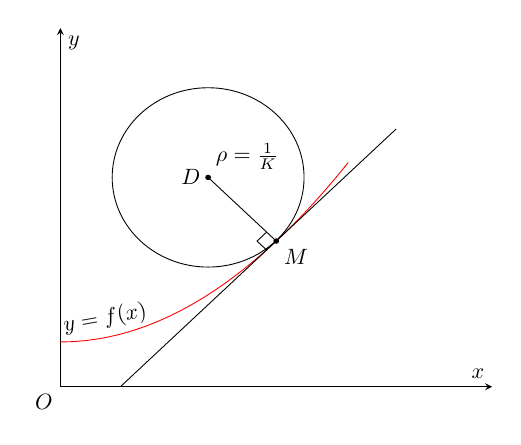
\begin{tikzpicture}[scale=0.8]
  \begin{axis}[clip=false,xmin=0, xmax=9,ymin=0,ymax=8, grid=none,
    xtick=\empty, ytick=\empty, axis lines=middle,
    smooth, xlabel={$x$}, ylabel={$y$}]

    % 曲线 y=f(x)
    % y' = 0.222 * x
    % y'' = 0.222
    \addplot[draw=red,domain=0:6] {x^2/9 + 1};

    % 弧段
    \node [above,rotate=10] at (1,1.11) {$y=f(x)$};
    \draw [fill] (4.5,3.25) circle [radius=0.05];
    \node [below right] at (4.5,3.25) {$M$};

    % 切线
    % y = x - 1.25
    \draw (1.25,0) -- (4.5,3.25) -- (7,5.75);

    % 曲率:K = 0.222 / (1+y'^2)^3/2 --> x = 4.5 --> K = 0.079
    % 半径:p = 1 / K = 12.73
    % 法线:y = -x + 7.75

    \draw [fill] (3.08,4.67) circle [radius=0.05];
    \draw (3.08,4.67) -- (4.5,3.25);
    \draw (3.08,4.67) circle [radius=2];
    \node [left] at (3.08,4.67) {$D$};
    \node [above right] at (3.08,4.67) {$\rho=\frac{1}{K}$};

    % y = -x + 7.35
    % y = x - 0.85
    \draw (4.3,3.05) -- (4.1,3.25) -- (4.3,3.45);

    % 原点
    \node [below left] at (0,0) {$O$};
  \end{axis}
\end{tikzpicture}

  \caption{曲率圆}
  \label{曲率圆}
\end{figure}

\paragraph{}
常常用曲率圆在点$M$邻近的一段圆弧来近似代替曲线弧,使问题简化。

\paragraph{}
按上述规定,曲线在点$M$处的曲率$K(k\neq0)$与曲线在点$M$处的曲率半径$\rho$有如下关系:
\begin{equation}
  \rho=\frac{1}{K}, \; K = \frac{1}{\rho}.
\end{equation}

\subsection{曲率中心的计算公式 渐屈线与渐伸线}
\paragraph{}
当点$(x,f(x))$沿曲线$C$移动时,相应的曲率中心$D$的轨迹曲线$G$称为曲线$C$的\uwave{渐屈线},而曲线$C$称为曲线$G$的\uwave{渐伸线}。所以曲线$y=f(x)$的渐屈线的参数方程为:

\begin{equation}
  \left\{\begin{array}{l}
    \alpha = x - \frac{y'(1+y'^2)}{y''} \\
    \beta = y + \frac{1+y'^2}{y''}
  \end{array} \right.
\end{equation}
其中$y=f(x), y'=f'(x),y''=f''(x), x$为参数,直角坐标系$\alpha O \beta$与$xOy$坐标系重合。

\begin{figure}[H]
\centering
  % involute aka evolvent
  % 渐屈线和渐伸线
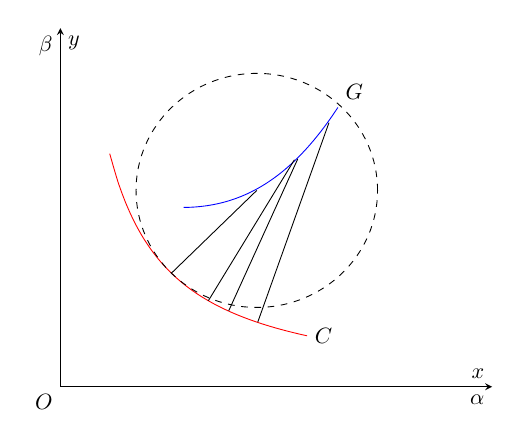
\begin{tikzpicture}[scale=0.8]
  \begin{axis}[clip=false,xmin=0, xmax=7,ymin=0,ymax=6, grid=none,
    xtick=\empty, ytick=\empty, axis lines=middle,
    smooth, xlabel={$x$}, ylabel={$y$}]

    \node [below left] at (0,6) {$\beta$};
    \node [below left] at (7,0) {$\alpha$};

    % 曲线 C
    % y' = -4/(x+0.2)^2
    % y'' = 8/(x+0.2)^3
    \node [right] at (4,0.85) {$C$};
    \addplot[draw=red,domain=0.8:4] {4/(x+0.2)-0.1};

    \node [above right] at (4.5,4.67) {$G$};
    \addplot[draw=blue,domain=2:4.5] {(x-2)^1.8/14*x + 3};

    \draw [dashed] (3.185,3.285) circle [radius=1.958];

    % (1.8,1.9)
    \addplot[domain=1.8:3.185] {x + 0.1};

    % (2.4,1.44)
    \addplot[domain=2.4:3.795] {1.69 * (x - 2.4) + 1.44};

    % (2.8,1.43)
    \addplot[domain=2.73:3.85] {2.27 * (x - 2.8) + 1.43};

    % (3.2,1.08)
    \addplot[domain=3.2:4.355] {2.89 * (x - 3.2) + 1.08};

    % 原点
    \node [below left] at (0,0) {$O$};
  \end{axis}
\end{tikzpicture}

  \caption{渐屈线和渐伸线}
  \label{渐屈线和渐伸线}
\end{figure}
